\documentclass[14pt]{beamer}

\usepackage{todonotes}
\usepackage{minted}
\usepackage{fontawesome}
\usetikzlibrary{arrows.meta}

\newcommand{\exturl}[1]{\exthref{#1}{#1}}
\newcommand{\exthref}[2]{\href{#1}{#2\ \footnotesize\faExternalLink}}

\beamertemplatenavigationsymbolsempty
\usecolortheme[dark]{solarized}
\setbeamertemplate{frametitle}[default][center]

\AtBeginSection{%
  \setbeamertemplate{headline}[default]
  \setbeamertemplate{footline}[default]
  \makeatletter\def\beamer@entrycode{\vspace*{-\headheight}}\makeatother
  \frame{\sectionpage}
  \setbeamertemplate{headline}[mine]
  \setbeamertemplate{footline}[mine]
}
\AtBeginSubsection{%
  \setbeamertemplate{headline}[default]
  \setbeamertemplate{footline}[default]
  \makeatletter\def\beamer@entrycode{\vspace*{-\headheight}}\makeatother
  \frame{\subsectionpage}
  \setbeamertemplate{headline}[mine]
  \setbeamertemplate{footline}[mine]
}

\defbeamertemplate{section page}{mine}[1][]{%
  \begin{centering}
    \vskip1em\par
    \begin{beamercolorbox}[sep=8pt,center,#1]{part title}
      \usebeamerfont{section title}\insertsection\par
    \end{beamercolorbox}
  \end{centering}
}
\setbeamertemplate{section page}[mine]
\defbeamertemplate{subsection page}{mine}[1][]{%
  \begin{centering}
    \vskip1em\par
    \begin{beamercolorbox}[sep=8pt,center,#1]{default}
      \usebeamerfont{section title}\insertsection\par
    \end{beamercolorbox}
    \begin{beamercolorbox}[sep=8pt,center,#1]{part title}
      \usebeamerfont{subsection title}\insertsubsection\par
    \end{beamercolorbox}
  \end{centering}
}
\setbeamertemplate{subsection page}[mine]

\defbeamertemplate{headline}{mine}[0]{%
  \leavevmode%
  \hbox{%
    \begin{beamercolorbox}[wd=\paperwidth,ht=3ex,center]{subsection title}
      \insertsectionhead\quad\quad\insertsubsectionhead
    \end{beamercolorbox}
  }
}
\defbeamertemplate{footline}{mine}[0]{%
  \leavevmode
  \hbox{%
    \begin{beamercolorbox}[wd=\paperwidth,center]{page number in head/foot}
      \usebeamerfont{page number in head/foot}\insertframenumber\par
    \end{beamercolorbox}
  }
}

\addtobeamertemplate{block begin}{}{\setlength{\parskip}{60pt plus 1pt
  minus 1pt}}

\author{Huon Wilson}
\title{\texttt{std::rand::random::<Talk>()}}
\begin{document}
\begin{frame}
  \maketitle
  \begin{center}
    \exturl{http://huonw.github.io/rand-dec14}
  \end{center}
\end{frame}

\section{Digital Randomness}
\begin{frame}
A sequence of bits, e.g.

\only<1>{\begin{equation*}
  11011110\,11111000\,01001010\,00111100\dots,
\end{equation*}

\phantom{.}

\vspace{2.5pt}

\phantom{.}}
\only<2>{\begin{equation*}
    \underbrace{11011110}_{\displaystyle 222}\underbrace{11111000}_{\displaystyle 248}
\underbrace{01001010}_{\displaystyle 74}\underbrace{00111100}_{\displaystyle 60}\dots,
  \end{equation*}
Usually generated/consumed in chunks.}

\end{frame}

\section{Why?}
\begin{frame}
  Lots of uses for randomness:
  \begin{itemize}
  \item simulations: scientific, testing
  \item games: shuffling cards, collecting loot
  \item security: keys, session IDs
  \end{itemize}

  All want ``high quality'' random numbers.
\end{frame}

\section{What is quality?}
\begin{frame}
  It depends!\\~\\

  Usually:

  \begin{itemize}
  \item uniformity: every bit has $50\%$ chance of being $0$ or $1$
  \item unpredictability: the value of a bit can't be guessed base
    on the value of others
  \end{itemize}
\end{frame}

\section{How can a deterministic machine be random?}
\begin{frame}
  Conventional computer RNGs follow patterns.
  \begin{center}
  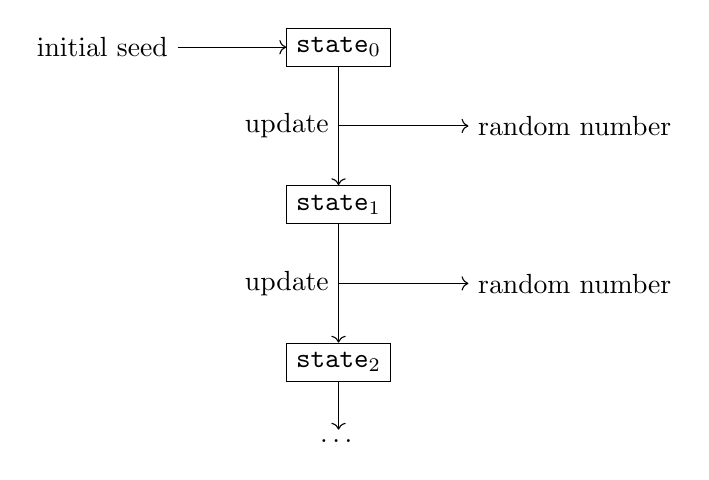
\begin{tikzpicture}
    \node (init) at (-3, 0) {initial seed};
    \node[draw] (State) at (0, 0) {\texttt{state}$_0$};
    \node[draw] (One) at (0, -2) {\texttt{state}$_1$};
    \node[draw] (Two) at (0, -4) {\texttt{state}$_2$};
    \node (dots) at (0, -5) {\dots};
    \node (Num1) at (3, -1) {random number};
    \node (Num2) at (3, -3) {random number};

    \draw[->] (init) -- (State);
    \draw[->] (State) -- (One) node[midway, left] {update};
    \draw[->] (One) -- (Two) node[midway, left] {update};
    \draw[->] (Two) -- (dots);
    \draw[->] (0, -1) -- (Num1);
    \draw[->] (0, -3) -- (Num2);
  \end{tikzpicture}
  \end{center}

  The seed controls \textit{which} pattern.
\end{frame}

\begin{frame}
  Compute the seed (or state), and you know the full stream. \\~\\

  RNGs for cryptography need to ensure the seed/state is hard to
  compute. (Or be true random number generators, e.g.~measure nuclear
  decay.) \\~\\

  Bad: XorShift. Good: ChaCha.
\end{frame}

\section{Rust}

\subsection[Thread-safety]{Thread-safety (by default)}
\begin{frame}
  Often a pervasive use of a single global RNG\@.
  Languages like C, R, Julia (recently improved in e.g. \exthref{https://github.com/JuliaLang/julia/pull/8832}{JuliaLang/julia\#8832}).\\~\\

  Automatically guaranteed this isn't a problem in Rust!
\end{frame}

\subsection{SIMD: dSFMT}
\begin{frame}[fragile]
  \fontsize{8pt}{8pt}\selectfont
  \begin{minted}{c}
__m128i v, w, x, y, z;

// ...
x = a->si;
z = _mm_slli_epi64(x, DSFMT_SL1);
z = _mm_xor_si128(z, b->si);
y = _mm_xor_si128(y, z);

v = _mm_srli_epi64(y, DSFMT_SR);
w = _mm_and_si128(y, sse2_param_mask.i128);
v = _mm_xor_si128(v, x);
v = _mm_xor_si128(v, w);
r->si = v;
u->si = y;
  \end{minted}

  \begin{flushright}
    \exthref{http://www.math.sci.hiroshima-u.ac.jp/~\%20m-mat/MT/SFMT/}{http://www.math.sci.hiroshima-u.ac.jp/\textasciitilde\ m-mat/MT/SFMT/}\\~\\
  \end{flushright}

\pause
  \begin{minted}{rust}
// ...
let y = (a << SSE2_SL) ^ b ^ y;
let v = (y >> SSE2_SR) ^ (y & SSE2_PARAMS_MASK) ^ a;

*r = v;
*u = y;
  \end{minted}

  \begin{flushright}
    \exturl{https://github.com/Grieverheart/dsfmt-rs}
  \end{flushright}

\end{frame}

\begin{frame}[fragile]
  Creates essentially the same ASM. Benchmark:\\~\\

\fontsize{10pt}{10pt}\selectfont
  \begin{minted}{rust}
let mut rng: dsfmt::DSFMTRng = SeedableRng::from_seed(12345u32);

let mut sum = 0_f64;
for _ in range(0u32, 1_000_000_000) {
    sum += rng.gen()
}

println!("{}", sum)
  \end{minted}

\begin{verbatim}
C
500014293.513722
User time: 1.86s
Rust
500014293.513722
User time: 1.93s
\end{verbatim}
\end{frame}

\subsection{Traits}
\begin{frame}[fragile]
  \begin{minted}{rust}
impl Rand for u8
impl Rand for u16
// ...
  \end{minted}

Get an number with a random value:

  \begin{minted}{rust}
use std::rand;

let x: u8 = rand::random();
let y: u16 = rand::random();
  \end{minted}
\end{frame}
\begin{frame}[fragile]
  \begin{minted}{rust}
impl Rand for XorShiftRng
impl Rand for ChaChaRng
// ...
  \end{minted}

Get an RNG with a random seed:

  \begin{minted}{rust}
use std::rand;

let x: rand::XorShiftRng = rand::random();
let y: rand::ChaChaRng = rand::random();
  \end{minted}
\end{frame}

\subsection{Community!}

\begin{frame}
  E.g.

  \begin{itemize}
  \item Careful analysis of documentation/use of
    \texttt{/dev/[u]random}
    \item Implement Bernstein's ChaCha RNG
      (\exturl{http://cr.yp.to/chacha.html}, sneves: \exthref{https://github.com/rust-lang/rust/pull/17387}{\#17387})
  \item Update \texttt{std::rand} to use the new, better
    \texttt{getrandom(2)} syscall on Linux, when available
    (strcat and klutzy: \exthref{https://github.com/rust-lang/rust/pull/18664}{\#18664})
  \end{itemize}
\end{frame}

\section{Questions?}
\end{document}

%%% Local Variables:
%%% mode: latex
%%% TeX-master: t
%%% TeX-command-extra-options: "-shell-escape"
%%% End:
